\chapter{UAV Navigation Using the RBL Algorithm and LiDAR Sensing\label{chap:lidar}}

    \section{Introduction}
        \subsection{Motivation}
        \ac{UAV}s are increasingly being deployed in challenging, unstructured environments like dense forests, moving beyond their traditional use in open areas.
        This shift is driven by a growing demand for autonomous solutions in sectors like environmental monitoring, forestry management (health assessment \cite{kurovec_fel_clanek}), and search and rescue, where ground-based access is difficult. 
        Furthermore, this work aligns with the broader trend of deploying \ac{UAV}s for increasingly complex tasks, such as detailed infrastructure inspection (e.g., power lines, where autonomous navigation in cluttered, potentially high \ac{EMI} environments is essential (Fly4Future \cite{f4f_powerline_inspection})). 
        Enabling UAVs to reliably navigate point-to-point within these challenging settings is a foundational step towards realizing these advanced applications safely and efficiently.

        While the primary objective of this work is to enable successful point-to-point navigation within a forest using the \ac{RBL} algorithm, a significant secondary benefit emerges from this process. 
        By successfully navigating from point A to point B while simultaneously building a map of the traversed environment, the UAV generates valuable spatial data about the forest structure. 
        This autonomously generated map can then serve a vital purpose: enabling enhanced planning for future missions within the same area. 
        Once a map exists, subsequent UAV operations could potentially transition from purely reactive navigation strategies to more efficient, globally informed path planning algorithms such as TODO find some. 
        Leveraging prior knowledge of obstacle locations could significantly improve the safety and efficiency of future routine tasks.
        
        \subsection{Problem Statement}
            Operating UAVs effectively within complex, three-dimensional environments like forests presents significant navigational challenges that hinder widespread autonomous deployment. 
            The primary problems addressed in this work stem from:
            \begin{enumerate}
                \item \textbf{\ac{GNSS}-Denied Conditions: } \\
                Within forests, the dense canopy and other obstructions frequently block or scatter \ac{GNSS} signals, leading to unreliable or completely absent reception.
                This necessitates reliance on onboard sensors and algorithms (like \ac{SLAM} based on \ac{LiDAR} and \ac{IMU} data) for accurate localization and state estimation.
                \item \textbf{Cluttered and Unpredictable Environments: } \\
                Forests are inherently cluttered with numerous static obstacles (trees, trunks, branches) and potentially dynamic ones (animals, leafs, falling branches). 
                The navigation system must be capable of perceiving these obstacles in real-time and planning safe paths around them without prior knowledge of their exact layout.
            \end{enumerate}
            Therefore, the core problem is to develop and validate a robust autonomous navigation system that allows a UAV to reliably traverse between specified points in a cluttered, GNSS-denied forest environment using only onboard sensing and computation.

        \subsection{Objectives}
            The primary objectives within this chapter are: 
            \begin{itemize}
                \item \textbf{Integrate the \ac{RBL} with Onboard Sensing: } \\
                    Adapt the core of the \ac{RBL} to utilize real-time sensor data. 
                    This includes modification of sensing cell $\mathcal{S}$, because used \ac{LiDAR} doesnt see in all directions. 
                    Sensing cell needs to remain convex so the centroid computed from partitioned cell $\mathcal{A}$ is never computed outside of the set - for safety convergence towards the goal.
                \item \textbf{Process Point Cloud Data: } \\
                    Implement neccessary filtration to refine the raw point cloud data acquired from the \ac{LiDAR}.
                \item \textbf{Integrate external packages on the \ac{UAV}: } \\
                    Integrate and configure external software packages for simultaneous environmental mapping and robust state estimation, suitable for operation within the \ac{GNSS}-denied forest environment.
                \item \textbf{Experimental and Simulation Validation: } \\
                    Conduct experiments to evaluate the performance, robustness, and effectiveness of the complete navigation solution. 
                    This validation will be performed first within a simulated forest environment and subsequently through real-world flight tests in an actual forest.
            \end{itemize}

        \subsection{Chapter Overview}
            TODO Summary of what this chapter covers

    \section{LiDAR-Based Perception and Point Cloud Processing}
        \subsection{Overview of LiDAR for UAV Navigation}
            \ac{LiDAR} is a crucial sensing technology widely used in applications such as SLAM \cite{pointlio_mrs}, autonomous vehicles \cite{Lidar_autonomous_vehicles}, UAVs TODOcite, and precision agriculture \cite{Lidar_agriculture}. 
            It provides high-resolution spatial data about the surrounding environment, making it a valuable tool for perception and navigation in dynamic and complex environments.  
            For UAV applications, \ac{LiDAR} serves several essential functions:  
            \begin{itemize}  
                \item \textbf{3D Mapping} -- Capturing a detailed representation of terrain, structures, and obstacles.  
                \item \textbf{Obstacle Detection} -- Identifying objects and estimating their position relative to the \ac{UAV} for collision avoidance.  
                \item \textbf{Autonomous Path Planning} -- Assisting navigation algorithms by providing spatial information for decision-making.  
                \item \textbf{Terrain Following} -- Helping the \ac{UAV} maintain a safe altitude by detecting variations in ground elevation.  
            \end{itemize}  

            \ac{LiDAR} offers several benefits that make it an attractive choice for \ac{UAV}-based navigation:  
            \begin{itemize}  
                \item \textbf{High Accuracy} -- Provides precise distance measurements, crucial for obstacle avoidance and localization.  
                \item \textbf{Environment Agnostic} -- Functions effectively in various conditions, including low-light environments and featureless terrain where cameras may fail.  
                \item \textbf{Fast Data Acquisition} -- Captures thousands to millions of points per second, enabling real-time processing.  
                \item \textbf{Rich Depth Information} -- Unlike cameras that provide only 2D images, \ac{LiDAR} generates accurate depth data, improving spatial awareness and 3D perception.  
            \end{itemize}  

            Despite its advantages, \ac{LiDAR} also presents certain challenges and limitations:  
            \begin{itemize}  
                \item \textbf{Computational Complexity} -- Processing large point clouds in real-time requires significant computational power, which may be a limitation for \ac{UAV}s with low processing resources.
                \item \textbf{Sensor Noise and Artifacts} -- External factors such as vibrations and motion of \ac{UAV} can introduce errors in point cloud data.  
                \item \textbf{Limited Field of View (FoV)} -- The placement of the \ac{LiDAR} sensor on the \ac{UAV} affects its coverage, requiring strategies to compensate for blind spots.  
                \item \textbf{Environmental Interference} -- Performance may degrade in challenging conditions such as fog, rain, or dense vegetation due light deviation.  
                \item \textbf{Power Consumption} -- \ac{LiDAR} sensors can consume a significant amount of power, which reduces the overall flight time of the \ac{UAV}.
                \item \textbf{Interference with Other LiDARs} -- \ac{LiDAR} sensors can experience interference when multiple units are used nearby, potentially leading to faulty measurements.
            \end{itemize}

        \subsection{Point Cloud Data Acquisition}
            \ac{LiDAR} systems determine object distances by emitting laser pulses and measuring the time it takes for the reflected light to return. 
            This process, known as \ac{ToF}, involves scanning the environment with laser beams directed at varying horizontal and vertical angles. 
            The reflected light, modulated in intensity, phase, or frequency, is captured by a receiver, which uses a lens to focus the signal onto a photodetector. 
            This detector converts the light into an electrical signal via the photoelectric effect \cite{lidar_how_works}.

            The system calculates distance based on the light's travel time, considering its near-light-speed propagation. 
            To distinguish transmitted from received signals, the laser's \setcounter{tocdepth}{1}
            wavelength is often adjusted. 
            Subsequent signal processing filters and analyzes the electrical signal, accounting for surface material and environmental variations. 
            The output is a 3D point cloud representing the scanned environment, along with reflected laser energy intensities. 
            All these data points are stored in a ROS message of type \(sensor\_msgs::PointCloud2\)

        \subsection{Preprocessing Techniques}
            To efficiently process \ac{LiDAR} data and reduce computational complexity, the raw point cloud undergoes downsampling and filtering. 
            The point cloud density is reduced using a voxel grid filter. 
            Subsequently, points associated with the \ac{UAV}'s structure are removed based on its known encumbrance.
            \begin{itemize}
                \item \textbf{Voxel Grid Downsampling} -- The raw \ac{LiDAR} point cloud often contains a large number of points, which can be computationally expensive to process in real-time. 
                To address this, we apply a voxel grid filter using the \ac{PCL} \cite{pcl_voxelgrid}. 
                This method partitions the 3D space into a grid of voxels with a given resolution (leafSize) and retains a single representative point per voxel. 
                The filtering process reduces the number of points while preserving the overall structure of the environment.
                \item \textbf{Filtering Points Corresponding to the UAV Structure} -- \ac{LiDAR} sensors mounted on \ac{UAV}s can capture unwanted points originating from the \ac{UAV} itself, such as reflections from its frame or rotor rods. 
                To prevent these points from interfering with navigation, additional filtering step has been applied.
                Points falling outside a specified distance range (closer than a minimum threshold or farther than a maximum threshold) are filtered out.
            \end{itemize}
            The resulting filtered point cloud contains only relevant environmental features while eliminating unnecessary points, improving efficiency for future processes.
            The point cloud is than fed into Point lio state estimator and bonxai mapping. TODO get access to repo.

        \subsection{Bonxai Mapping}
            As will be shown later in this chapter, prior terrain knowledge is beneficial for navigation. 
            For this purpose, environmental mapping was accomplished using a simple package developed by the MRS group, implementing the Bonxai mapping approach.
            The resulting map is represented as a voxel grid, which is then used by the \ac{RBL} algorithm for navigation planning.

            Initially, an approach involving surface reconstruction from this voxel data was investigated. 
            This involved estimating surface normals from the point cloud combined with Greedy Projection Triangulation (GP3) method from the PCL library to generate polygonal mesh approximating the environment's surface.
            While this method could produce relatively accurate surface representation, it turned out to be computationally expensive and too slow for real-time execution on the \ac{UAV}'s onboard computer.

            Due to these limitations, the surface reconstruction approach was abandoned. Instead a simpler and more efficient method was adopted, which involves directly using the information about the environment stored in voxel grid map.
            This direct voxel usage approach is detailed in the subsequent section. 
            Consequently, further development of the mesh-based surface reconstruction method is not recommended for this application.

        \subsection{Directly using voxels to modify cell A}
            
    
        \subsection{Using the found closest points for cell A partition}
            \subsection{Finding the Closest Point on a Triangle}
            \subsection{Plane Calculation for Slicing Cell A}
            \subsection{Integration with the RBL Algorithm}

    \section{Implementation and Integration on UAV}
        TODO
        \subsection{Challanges in Integration}
            \begin{figure}[htbp]
                \centering
                \subfloat[UAV model with visualized LiDAR mounting parameters.] {
                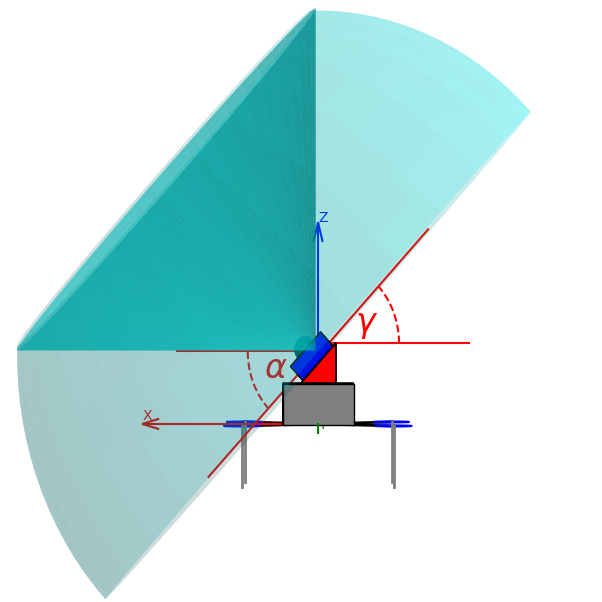
\includegraphics[width=0.48\textwidth]{./fig/photos/uav_side_view.png}
                \label{fig:model_uav}
                }
                \subfloat[UAV used in the experiment with mounted LiDAR] {
                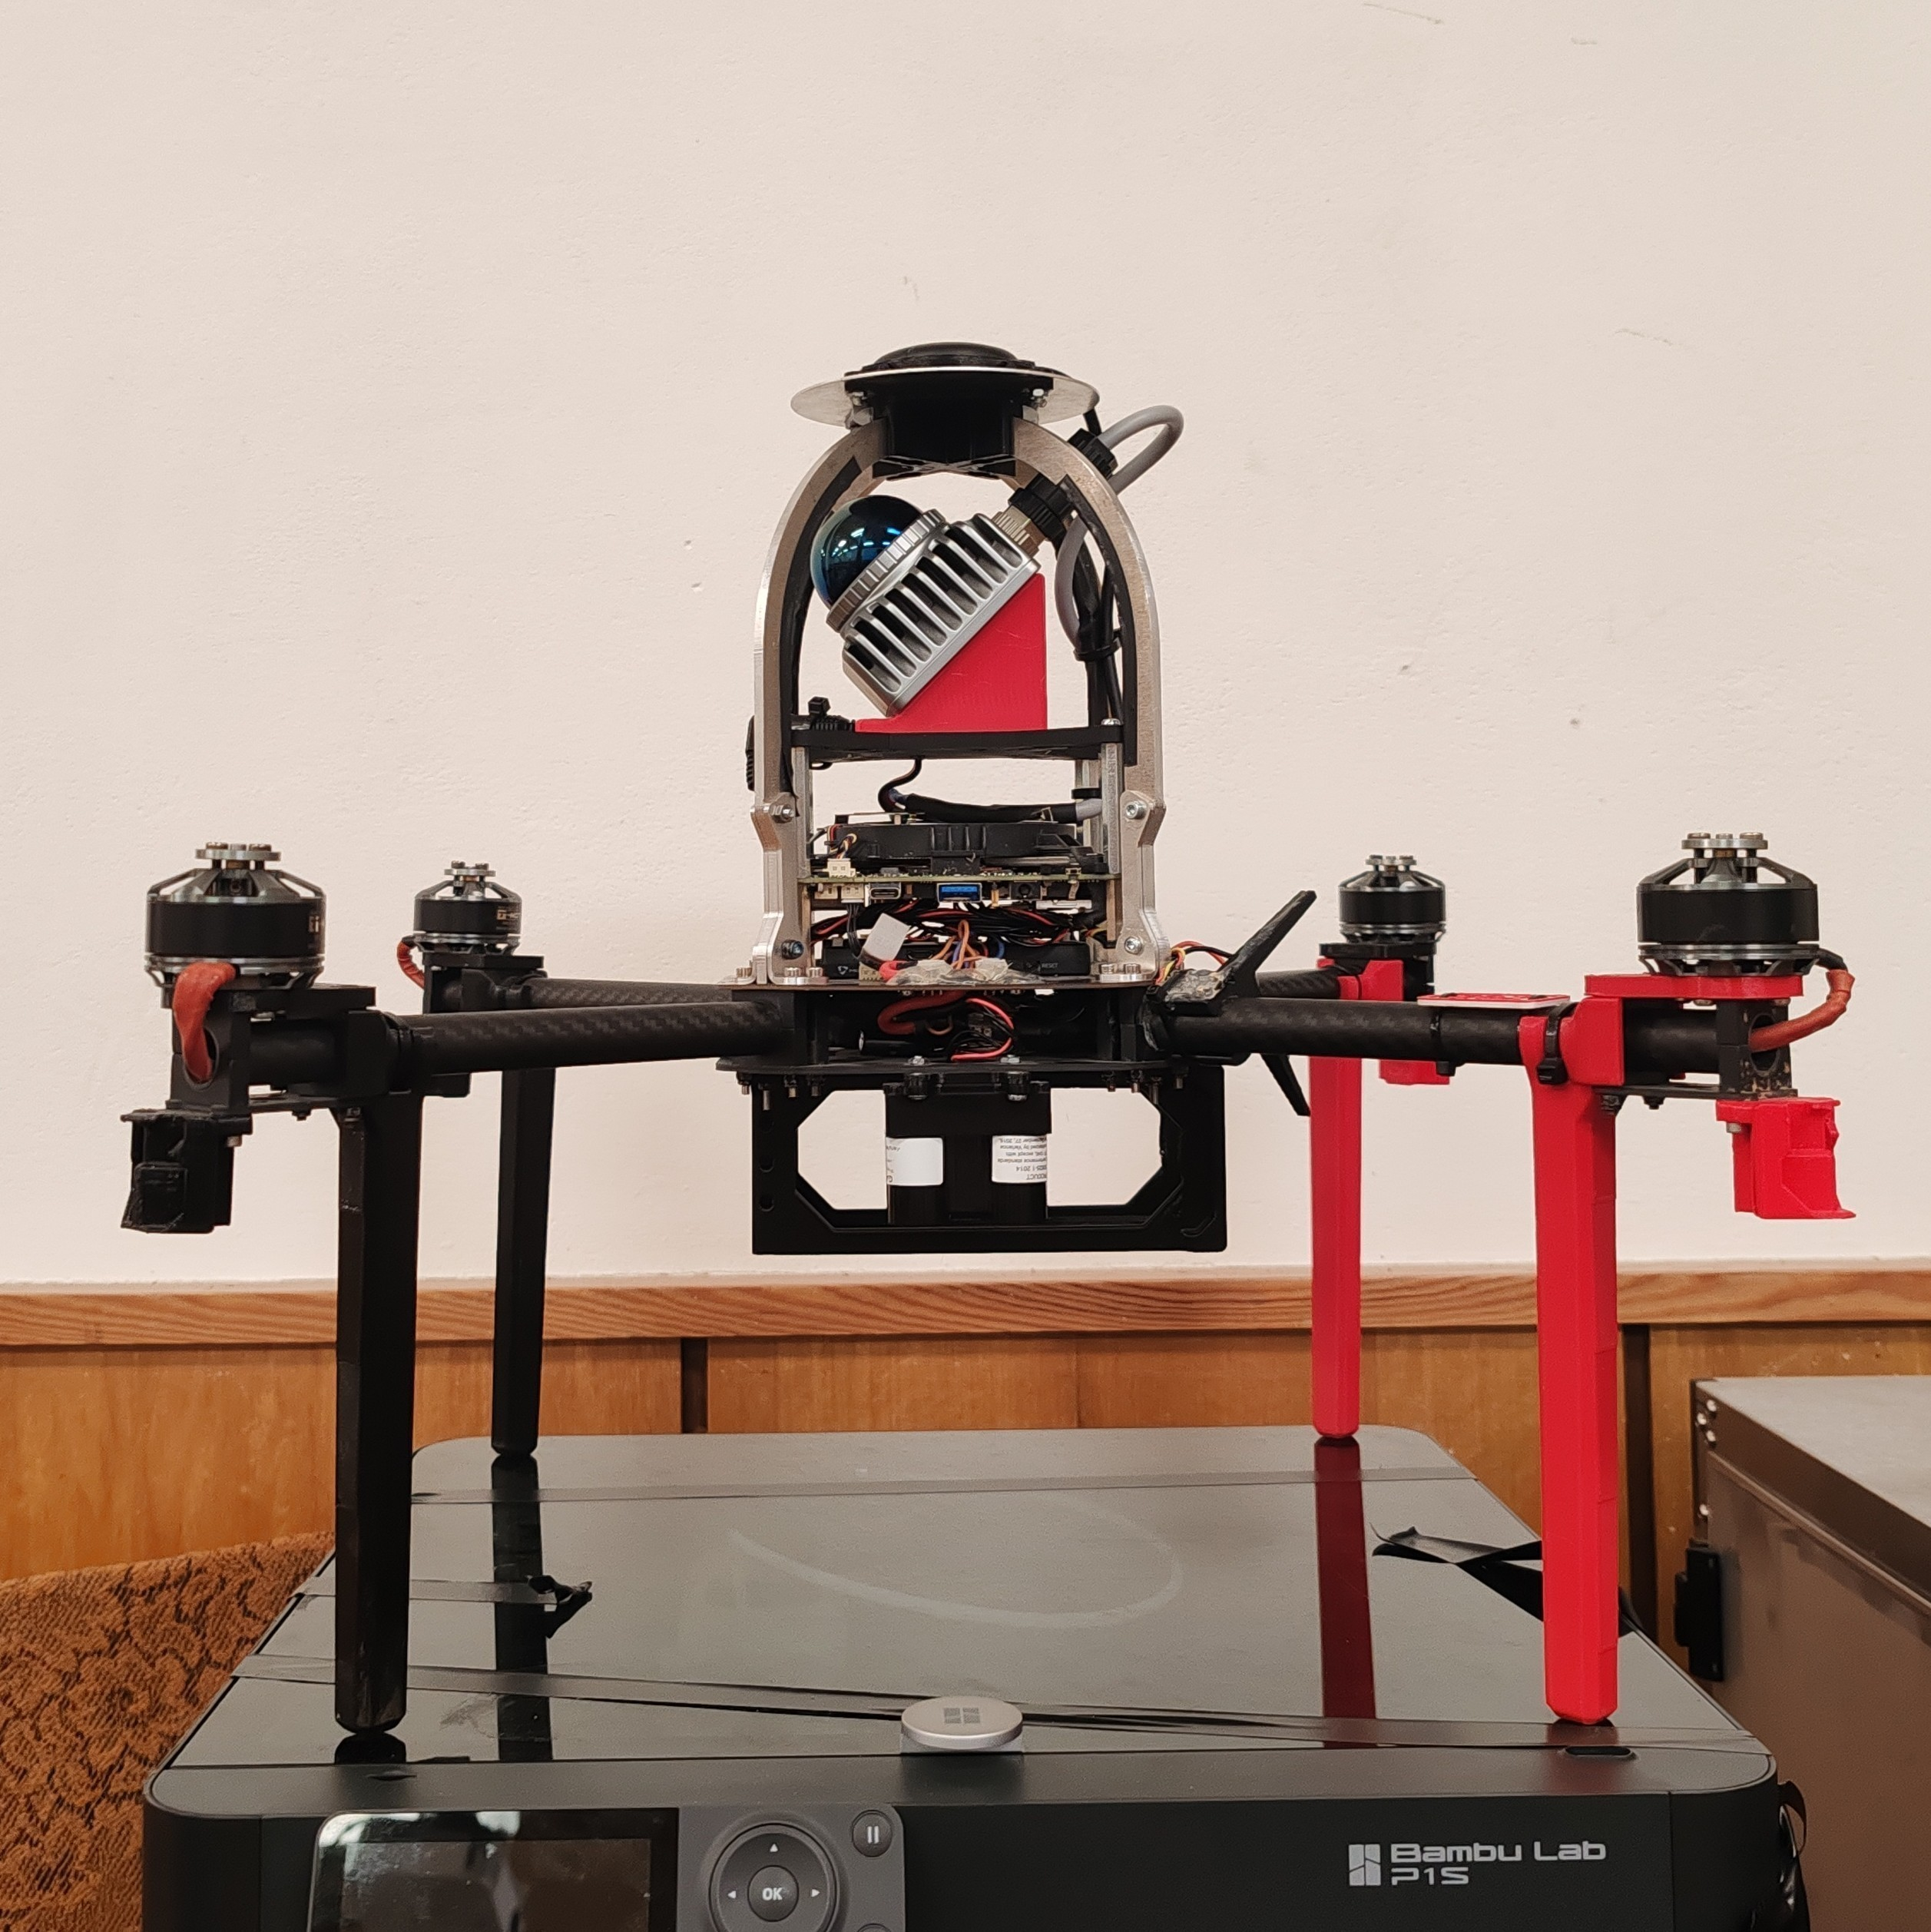
\includegraphics[width=0.48\textwidth]{./fig/photos/uav_photo.jpg}
                \label{fig:uav_1}
                }
                \caption{
                    UAV and LiDAR mounting scheme.
                    Subfigure (a) shows a modeled UAV with visualized LiDAR mounting parameters, including the LiDAR elevation field of view $\alpha$ and tilt angle $\gamma$. 
                    Subfigure (b) displays the real UAV used in the experiment with the LiDAR mounted according to the same configuration.                                                
                }
                \label{fig:uavs}
            \end{figure}

            For modification of cell A 2 planes are defined using real knowledge of how LiDAR is mounted on the uav and livox vertical fov
            Let $\mathbf{e}_z = \begin{bmatrix} 0 \\ 0 \\ 1 \end{bmatrix}$ be the unit vector along the z-axis,  
            $R_{\text{off}} \in SO(3)$ the offset rotation, and  
            $R_{\text{rpy}} \in SO(3)$ the roll-pitch-yaw rotation. 
            $\alpha_1$, $\alpha_2$, $\alpha_3$

            Then the resulting vector is given by:  
            \[
            \mathbf{n} = R_{\text{rpy}} \cdot R_{\text{off}} \cdot \mathbf{e}_z
            \]

            Modified cell S:
            \begin{equation}
                \mathcal{S}_i = {} 
            \end{equation}
            livox - 360 * 60 deg - account for centroid calculation
        \subsection{Software and Hardware setup}
            LiDAR sensor config, uav platform specifications
    
    \section{Simulation and Experimental Results}
        TODO
        \subsection{Simulation Setup}
            virtual environment modeling, tools used
        \subsection{Performance in Simulated Environments}
            Success rates, obstacle avoidance, efficiency metrics - same as in the rbl
        \subsection{Real-World Experiments in a Forest Environment}
        \subsection{Comparative Analysis}
            Simulation vs. real-world performance
    
    \section{Conclusion}
        TODO
        Summary of contributions and some directions for future research
    








        % \subsection{Surface Reconstruction and Triangulation}
        %     The map has been used for surface reconstruction:
        %     To obtain a continuous surface representation from the point cloud, normal estimation and triangulation are performed. 
        %     This process involves estimating surface normals, combining them with point positions, and applying a triangulation algorithm to generate a polygonal mesh.
        %     \begin{itemize}
        %         \item \textbf{Normal Estimation: } \\ 
        %         Surface normals are estimated using the Point Cloud Library (PCL) TODOcite. 
        %         A k-d tree is employed to efficiently find neighboring points, and the normal at each point is computed based on its local neighborhood. 
        %         This provides information about the surface curvature and orientation.
        %         \item \textbf{Point Cloud and Normal Merging: } \\ 
        %         Once the normals are estimated, they are combined with the original point cloud to create a representation that includes both spatial position and surface orientation.
        %         \item \textbf{Triangulation Using Greedy Projection: } \\
        %         The point cloud is converted into a polygonal mesh using the Greedy Projection Triangulation (GP3) method. 
        %         This algorithm forms triangles between neighboring points while enforcing constraints on edge length, surface angles, and normal consistency. 
        %         A k-d tree is used to accelerate the search for nearest neighbors, ensuring efficient mesh generation.
        %         \item \textbf{Results: } \\ 
        %         The output is a polygonal mesh that approximates the underlying surface of the point cloud. 
        %         This mesh can be used for visualization and obstacle avoidance.
        %     \end{itemize}
        %     This has been tried, but turned out to be unnecessary computationally expensive and on the UAV onboard computer slow. 
        %     It was able to approximate surface of its surrounding semi-well. 
        %     But due for it being slow a simplier method have been used - (Directly using voxels to modify cell A) instead of aporximating surface.
        %     So I just wanted to quiky say that this was tested, unsuccesflully so no future development of this methos is recomended or something like that. 


        %     There will be picture from rviz how it approximated surface.
